\textit{Before using the data, a level of data processing should be applied to ensure a workable dataset for the \gls{lfp} and \gls{imu}-based algorithms. This applies differently to the different data from the dataset and is concerned with both formatting and cleaning the data.}

\section{Data Processing Flow}
As mentioned in \textbf{\autoref{sec:data}}, we have decided to work with the dataset provided by the Indoor Location \& Navigation Competition. This dataset contains four folders of data, where all the files within the file structure are regular text files (.txt). Since the purpose of each folder is different, as well as the file structure, different levels of formatting and cleaning is needed.

\begin{figure}[H]
    \centering
    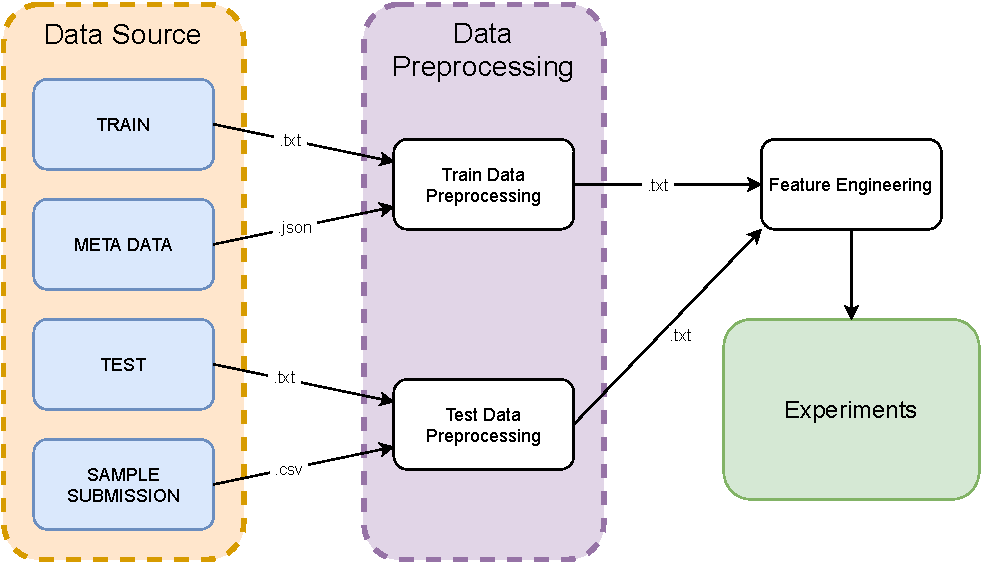
\includegraphics[scale=0.7]{Images/DataStandard/DataArch.pdf}
    \caption{The overall architecture of data processing components.}
    \label{fig:DataArchitecture}
\end{figure}

To determine how to prepare the data for the algorithms, we created an overall architecture of the data processing, which can be viewed on \textbf{\autoref{fig:DataArchitecture}}. The three different components, namely \textit{Data Preprocessing}, \textit{Feature Engineering} and \textit{Test Preprocessing}, will be described in the following sections.

%The \textit{Data Preprocessing} will be divided into two parts: \textit{Train Data Conversion} and \textit{Train Data Cleaning}.

\subsection{Libraries}
To work with the data preprocessing and pipeline, we utilise Python as the programming language. For the \textit{Test Data Preprocessing} and \textit{Data Pipeline} the library Pandas\cite{pandas} has been used to manipulate the data. The Pandas library requires the library NumPy\cite{numpy}. These libraries offer data structures and operations for the needed data manipulation.
The \textit{Data Pipeline} uses the Counter library from the Collection module from the Python Standard Library to organise and filter the \gls{bssid}s and make a directory to get easy access to the relevant beacons/Wi-Fi points.
%Python, pandas etc

\subsection{Train Data Preprocessing}
The \textit{Train Data Preprocessing} is supposed to be executed once where the result of this execution are text files representing each path in the training data. The data are split to have the waypoints accessible to the pipeline without an overhead in the processing of the files. The new files are structured to minimise the need to analyse the files in the feature engineering. This process will further be elaborated on in \textbf{\autoref{sec:dataPreprocessing}}.

\subsection{Feature Engineering} \label{sec:datapipeline}
After preprocessing, the data should be formatted according to the usage of the specific methods, which is depicted in \textbf{\autoref{fig:DataArchitecture}} as \textit{Feature Engineering}. The \textit{Feature Engineering} phase therefore takes the general processed data and transforms it to the format for the four types of experiments: There is one type for the \gls{imu}-based algorithms and two for \gls{lfp} methods, either making use of time series or not, and one for the hybrid.

\subsection{Test Data Preprocessing}
When the algorithms and models are ready to be tested against the test data from the competition, the test data is desired to be structured similarly to the train data after preprocessing. \textit{Test Data Preprocessing} combines the data from the \textit{TEST} folder and the \textit{sample\_submission.csv}, as seen \textbf{\autoref{fig:DataArchitecture}}, to create similar looking files to the outcome of the \textit{Train Data Preprocessing} phase. 
%This would then make it easier to evaluate the algorithms and models, which will happen by uploading the results of the location estimates of the test dataset to the Kaggle competition, which in return will output the evaluation of the test dataset. 
This process will be further elaborated on in \textbf{\autoref{sec:dataPreprocessing}}.

\section{Data Preprocessing}
\label{sec:dataPreprocessing}
This section describes the \textit{Data Preprocessing} component depicted on \textbf{\autoref{fig:DataArchitecture}} in detail. The first folder in the \textit{Data Source} is the \textit{TRAIN} folder, which contains files on the regular text format, which we want to format differently. The reason for this is to more easily work with the data. Additionally, we have chosen to remove the file structure, which first partitions the data into site and then floor level to instead simply add this information within each new \textit{.txt} file.

A level of data cleaning should also be executed in the \textit{Train Data Preprocessing} phase. This is among others concerned with normalising the floor level format to the same as the submission format, which should be integers. This is due to floors being denoted in the dataset either as "\textit{F1}", "\textit{1F}" or "\textit{L1}". Therefore, to standardise the floor levels, we have normalised this to "0" for all of the previous cases. In the metadata, most of the floors have been defined as an integer. In case the floors are above ground level, the floor value must be subtracted by one, because of the way it has been illustrated in the metadata. The floors that are not available in the metadata have been converted manually from the known values to the desired integer value. When adding the manual conversion, every floor is convertible, meaning that this operation does not exclude any data.

%Problemet med new lines
%In the training files, you may find occasionally that a line is missing the ending newline character, causing it to run on to the next line. It is up to you how you want to handle this issue. This issue is not found in the test data.
%Additionally, as mentioned in \textbf{\autoref{sec:dataset}}, there is missing some new line characters in the dataset. This issue is handled by l
%Outlier detection and removal such as looking whether the accelorometer values are proper.

%In the \gls{json} files the redundant data will be removed to minimise the size of each file. %Skal uddybes hvad er
At the beginning of each file, a variety of information was displayed. Most of this was removed since it was redundant for the experiments we are to conduct. Now, only site ID, site name and path ID are stored at the beginning of each file. All this formatting and cleaning would result in \textit{.txt} files with a similar structure to \textbf{\autoref{fig:newformat}}.

%The reason for this conversion is that \gls{json} is a universal data object format, supported by most languages by default or by adding a library. Additionally, we have chosen to remove the file structure, which first partitions the data into site and then floor level to instead simply add this information within each new \gls{json} file. This would result in \gls{json} files with a similar structure to \textbf{\autoref{fig:jsonformat}}.

\begin{figure}[H]
\lstset{numbers=left}
\begin{lstlisting}[language=Python]
#	5a0546857ecc773753327266
#	Xixi Yintai City
#	5d134069ffe23f000860512b
[...]273    TYPE_WAYPOINT                   [WAYPOINT 1]	  [WAYPOINT 2]      ...
[...]425    TYPE_ACCELEROMETER	            -1.1477051      1.6084747	        ...
[...]425    TYPE_MAGNETIC_FIELD	            9.970093        31.666565	        ...
[...]425    TYPE_GYROSCOPE	                0.23286438      -0.18293762	      ...
[...]425    TYPE_ROTATION_VECTOR            0.09658819	    0.061834227       ...
[...]425    TYPE_MAGNETIC_FIELD_UNCALI..    -95.12787	      -39.694214        ...
[...]425    TYPE_GYROSCOPE_UNCALI..	        0.2890625	      -0.26670837       ...
[...]425    TYPE_ACCELEROMETER_UNCALI..	    -1.1441193	    1.7066345         ...

...

#	1561454731737
\end{lstlisting}
\caption{The \textit{.txt} format we have converted the data into.}
\label{fig:newformat}
\end{figure}
%begin{figure}[H]
%\lstset{numbers=left}
%\begin{lstlisting}
%{ 
    %siteID:
    %siteName:
    %floorLevel:
    %pathID:
    %startTime:
    %sensorData: 
        %[
            %{
                %attributesFromKaggle
                %label { x, y } // closest waypoint
            %},
            %{
                %attributesFromKaggle
                %label { x, y } // closest waypoint
            %},
            %...
       %]
%}
%\end{lstlisting}
%\caption{The \gls{json} format we have converted the data into.}
%\label{fig:jsonformat}
%\end{figure}

\textbf{\autoref{fig:newformat}} displays the formatted data. Similar to the previous structure, the file is of \textit{.txt} format and the attributes on each line is tab-separated. Each file contains information about site ID (\textit{line 1}), site name (\textit{line 2}), and path ID (\textit{line 3}).

%floor level the specific path has been measured at, alongside the ID of the path and a timestamp of when the measurement has begun.

On \textit{line 4} to \textit{line 11}, we see the data on a similar format to the data provided by Indoor Location \& Navigation Competition. Each entry is first described by a timestamp. The second field indicates the type of data, where \textit{line 4} is the data of type waypoint. This has been restructured from the original, where each tab-separated field after the '\textit{TYPE\_WAYPOINT}' is a waypoint from this path. The reason for gathering the waypoints at the top of the file is to make it easily accessible (for example when extracting the ground truth data). The timestamp on \textit{line 4} indicates the start time for the path. Thereafter, it includes all the sensor measurements similar to the original dataset. Lastly, each file contains the end time of the path.

\begin{figure}[H]
\lstset{numbers=left}
\begin{lstlisting}[language=Python]
1561454339274,1,78.25796,11.443387
\end{lstlisting}
\caption{An example of a waypoint.}
\label{fig:waypointformat}
\end{figure}

On \textbf{\autoref{fig:newformat}} \textit{line 4}, the different waypoints have been abstracted away. An example of one of these waypoints can be viewed on \textbf{\autoref{fig:waypointformat}}, which displays both the structure and content of a waypoint. The waypoints objects are comma-separated and contain four values, namely timestamp, floor level, X-coordinate and Y-coordinate.

%Lastly is an array containing the different sensor observations from the original path file. Each observation contains the original attributes, and we have determined and added the closest waypoint to each observation. The closest waypoint is determined by the timestamps meaning that the x- and y-coordinates for a sensor measurement are determined by the waypoint which is closest to the measurement. 
